%%%%%%%%%%%%%%%%%%%%%%%%%%ch3-2
\begin{frame}[shrink]
  \frametitle{ch3.信号检测与估计理论的基础知识}
  \framesubtitle{ch3-2. 贝叶斯准则}
  \tableofcontents[hideallsubsections]
\end{frame}

\section{贝叶斯准则}

\begin{frame}{贝叶斯准则---基本要求}
\begin{itemize}
	\item 充分理解平均代价(Average risk)的概念
	\item 贝叶斯准则(Bayes criterion)的判决表达式
	\item 判决性能分析
\end{itemize}

\bigskip
\textcolor{blue}{贝叶斯准则的基本原理:在划分观察空间时,使平均代价最小。}
\end{frame}

\begin{frame}{信号统计检测理论要研究的基本问题---判决域的划分}
\begin{columns}
	\column{0.5\textwidth}
	\begin{align*}
	&H_0: x=-A+n,\quad H_1: x=A+n\\
	&H_0: x_k=-A+n_k,\quad H_1: x_k=A+n_k\\
	&k=1,2,\dots,N,\quad \bm{x}=(x_1,x_2,\dots,x_N)^{T}\\
	&P(H_i|H_j)=\int_{R_i}p(\bm{x}|H_j)d\bm{x}
	\end{align*}
	\column{0.5\textwidth}
	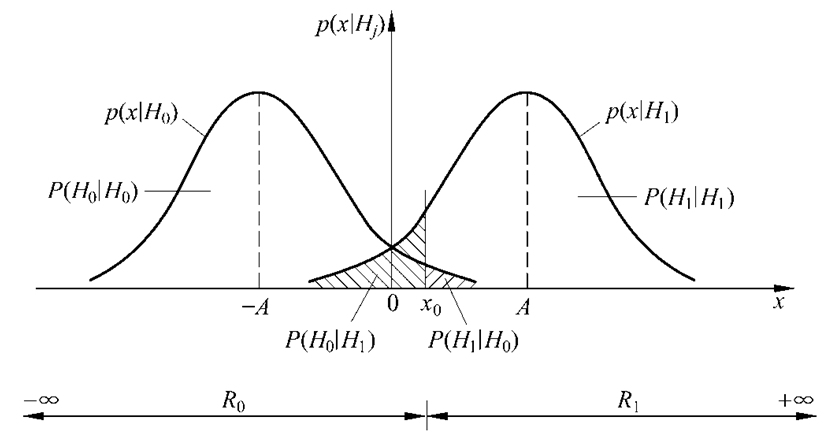
\includegraphics[scale=0.4]{detectionA}
\end{columns}
\begin{itemize}
	\item 目标: 正确判决概率$P(H_j|H_j)$尽可能大,错误判决概率$P(H_i|H_j)(i\ne j)$尽可能小。
	\item 判决域的划分影响判决概率$P(H_i|H_j)$, 因此\textbf{需要最佳划分判决域}。
	\item $p(\bm{x}|H_j)(j=0,1)$: 假设$H_j$下观测信号的概率密度函数。它描述观测(接收)信号的统计特性。
	\item 按照一定的准则,将观察空间$\bm{R}$分别划分为$R_0$和$R_1$两个子空间。
	计算判决概率$P(H_i|H_j)(i,j=0,1)$。	
\end{itemize}
\end{frame}

\begin{frame}{贝叶斯检测的提出动机}
通信系统中, 二元信号的平均解调错误概率(由全概率公式得出):
\[ P_e=P(0)P(1|0)+P(1)P(0|1)\]
可以看出, 检测性能不仅与两种错误判决概率$[P(1|0),P(0|1)]$有关, 还与信源发送的0和1的先验概率$[P(0),P(1)]$有关。\\
另外, 没做出一种判断, 人们要付出的代价也是不同的。\\
如何综合考虑上述因素来设计好的检测方法?
\begin{block}{贝叶斯检测}
	给定各种判决代价因子, 且已知各假设的先验概率条件下,使\textbf{平均代价最小}的检测准则。
\end{block}
\end{frame}

\begin{frame}{问题}
\begin{enumerate}
	\item 代价因子如何定义?
	\item 平均代价如何计算?
	\item 如何获得最小的平均代价?
\end{enumerate}
\end{frame}

\begin{frame}{代价因子的定义}
\begin{block}{对于二元信号统计检测, 共有四种事件发生, 即}
$$
\begin{array}{cccc}
	(H_0|H_0) & (H_1|H_0) & (H_1|H_1) & (H_0|H_1)\\
	\Downarrow & \Downarrow & \Downarrow & \Downarrow\\
	c_{00} & c_{10} & c_{11} & c_{01}
\end{array}
$$
$c_{ij}$表示假设$H_j$为真时, 判决假设$H_i$成立所付出的代价
\end{block}
\begin{block}{Notes}
	一般地, $c_{10}>c_{00}, c_{01}>c_{11}$
\end{block}
\end{frame}

\begin{frame}{平均代价的计算}
\begin{block}{平均代价$C$由两部分构成}
	\begin{enumerate}
		\item 信源发送$H_0$假设时, 判决所付出的代价$C(H_0)$
		\item 信源发送$H_1$假设时, 判决所付出的代价$C(H_0)$
	\end{enumerate}
    \[C=P(H_0)C(H_0)+P(H_1)C(H_1)\]
\end{block}
参见:
\[ P_e=P(0)P(1|0)+P(1)P(0|1)\]
\end{frame}

\begin{frame}{平均代价的计算}
\begin{block}{对于二元信号统计检测, 共有四种事件发生, 即}
	$$
	\begin{array}{cccc}
	(H_0|H_0) & (H_1|H_0) & (H_1|H_1) & (H_0|H_1)\\
	\Downarrow & \Downarrow & \Downarrow & \Downarrow\\
	c_{00} & c_{10} & c_{11} & c_{01}
	\end{array}
	$$
	$c_{ij}$表示假设$H_j$为真时, 判决假设$H_i$成立所付出的代价
\end{block}
\begin{block}{因此, 两种假设下, 判决所付出的代价: }
   \begin{align*}
   C(H_0)&=c_{00}P(H_0|H_0)+c_{10}P(H_1|H_0)\\
   C(H_1)&=c_{01}P(H_0|H_1)+c_{11}P(H_1|H_1)
   \end{align*}
\end{block}
 平均代价: $C=P(H_0)C(H_0)+P(H_1)C(H_1)$
\end{frame}

\begin{frame}{平均代价的计算}
\begin{align*}
C&=P(H_0)C(H_0)+P(H_1)C(H_1)\\
C(H_0)&=c_{00}P(H_0|H_0)+c_{10}P(H_1|H_0)\\
C(H_1)&=c_{01}P(H_0|H_1)+c_{11}P(H_1|H_1)
\end{align*}
\centering $\Downarrow$
\begin{align*}
C=&P(H_0)c_{00}P(H_0|H_0)+c_{10}P(H_1|H_0)+\\
&P(H_1)c_{01}P(H_0|H_1)+c_{11}P(H_1|H_1)
\end{align*}
\end{frame}

\begin{frame}[shrink]{平均代价的计算}
\begin{columns}
	\column{0.55\textwidth}
	\begin{align*}
	C=&P(H_0)c_{00}P(H_0|H_0)+c_{10}P(H_1|H_0)+\\
	&P(H_1)c_{01}P(H_0|H_1)+c_{11}P(H_1|H_1)
	\end{align*}
	\[ P(H_i|H_j)=\int_{R_i}p(x|H_j)dx\]
	\column{0.35\textwidth}
	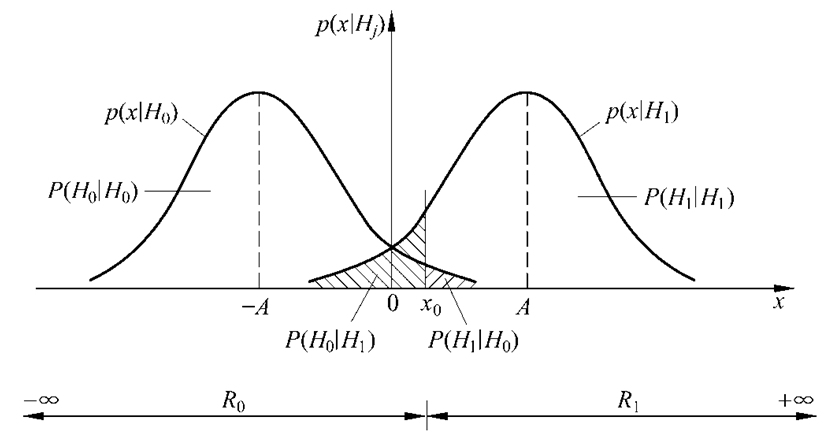
\includegraphics[scale=0.35]{detectionA}
\end{columns}

\medskip
\centering $\Downarrow$
\begin{align*}
C=&P(H_0)\left(c_{00}\int_{R_0}p(x|H_0)dx+c_{10}\int_{R_1}p(x|H_0)dx\right)+\\
&P(H_1)\left(c_{01}\int_{R_0}p(x|H_1)dx+c_{11}\int_{R_1}p(x|H_1)dx\right)
\end{align*}

\end{frame}

\begin{frame}[shrink]{平均代价的计算}
\begin{columns}
	\column{0.7\textwidth}
	\begin{align*}
	C=&P(H_0)\left(c_{00}\int_{R_0}p(x|H_0)dx+c_{10}\int_{R_1}p(x|H_0)dx\right)+\\
	&P(H_1)\left(c_{01}\int_{R_0}p(x|H_1)dx+c_{11}\int_{R_1}p(x|H_1)dx\right)
	\end{align*}
	\[\int_{R}p(x|H_j)dx=1 \implies \int_{R_1}p(x|H_j)dx=1-\int_{R_0}p(x|H_0)dx \]
	\column{0.3\textwidth}
	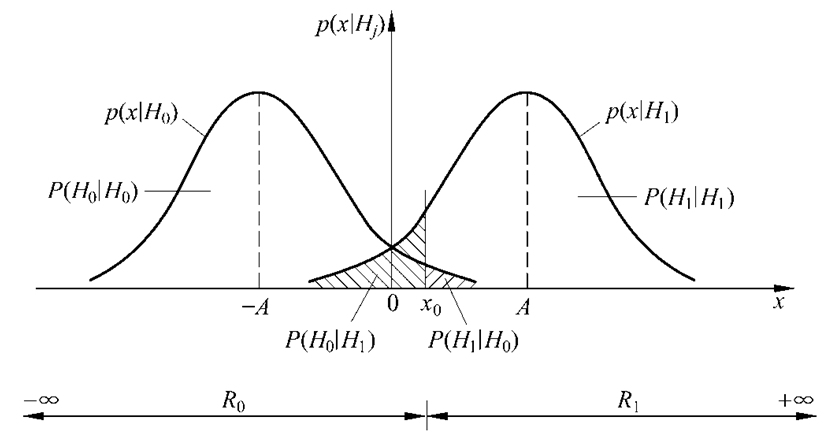
\includegraphics[scale=0.27]{detectionA}
\end{columns}

\medskip
\centering $\Downarrow$
\begin{align*}
C=&P(H_0)\left(c_{00}\int_{R_0}p(x|H_0)dx+c_{10}\left(1-\int_{R_0}p(x|H_0)dx\right)\right)+\\
&P(H_1)\left(c_{01}\int_{R_0}p(x|H_1)dx+c_{11}\left(1-\int_{R_0}p(x|H_1)dx\right)\right)
\end{align*}
\end{frame}

\begin{frame}[shrink]{平均代价的计算}
\begin{align*}
C=&P(H_0)\left(c_{00}\int_{R_0}p(x|H_0)dx+c_{10}\left(1-\int_{R_0}p(x|H_0)dx\right)\right)+\\
&P(H_1)\left(c_{01}\int_{R_0}p(x|H_1)dx+c_{11}\left(1-\int_{R_0}p(x|H_1)dx\right)\right)\\
=&P(H_0)\left(c_{10}+c_{00}\int_{R_0}p(x|H_0)dx-c_{10}\int_{R_0}p(x|H_0)dx\right)+\\
&P(H_1)\left(c_{11}+c_{01}\int_{R_0}p(x|H_1)dx-c_{11}\int_{R_0}p(x|H_1)dx\right)\\
=&c_{10}P(H_0)+c_{11}P(H_1)+\\
&\left(\int_{R_0}\left[P({H_1})(c_{01}-c_{11})p(x|H_1)-P(H_0)(c_{10}-c_{00})p(x|H_0)\right]dx \right)
\end{align*}
\end{frame}

\begin{frame}[shrink]{平均代价取最小的条件}
\begin{align*}
C=&c_{10}P(H_0)+c_{11}P(H_1)+\\
&\left(\int_{R_0}\left[P({H_1})(c_{01}-c_{11})p(x|H_1)-P(H_0)(c_{10}-c_{00})p(x|H_0)\right]dx \right)
\end{align*}
\begin{columns}
	\column{0.46\textwidth}
	$c_{10}P(H_0)$和$c_{11}P(H_1$是两项固定的值\\
	$P({H_1})(c_{01}-c_{11})p(x|H_1)\ge 0$\\
	$P(H_0)(c_{10}-c_{00})p(x|H_0)\ge 0$
	\column{0.35\textwidth}
	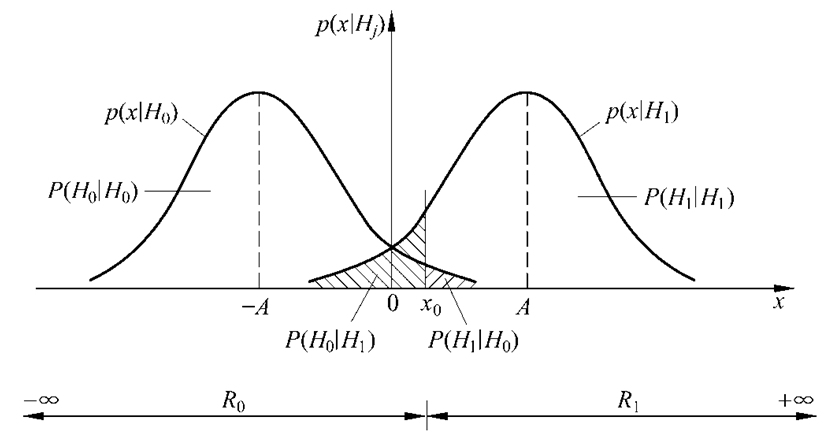
\includegraphics[scale=0.35]{detectionA}
\end{columns}
\begin{itemize}
	\item \textcolor{blue}{\textbf{因此, 给定信道特性和先验信息, 平均代价$C$的大小完全由判决域$R_0$确定。}}
	\item \textbf{把被积函数取负值的观测值$x$划分给$R_0$区域, 而把其余的观测值$x$划分给$R_1$, 即可保证平均代价最小。}
\end{itemize}
\end{frame}

\begin{frame}[shrink]{平均代价取最小的条件}
\begin{align*}
C=&c_{10}P(H_0)+c_{11}P(H_1)+\\
&\left(\int_{R_0}\left[P({H_1})(c_{01}-c_{11})p(x|H_1)-P(H_0)(c_{10}-c_{00})p(x|H_0)\right]dx \right)
\end{align*}
\begin{columns}
	\column{0.46\textwidth}
	\textbf{把被积函数取负值的观测值$x$划分给$R_0$区域, 而把其余的观测值$x$划分给$R_1$, 即可保证平均代价最小。}
	\column{0.35\textwidth}
	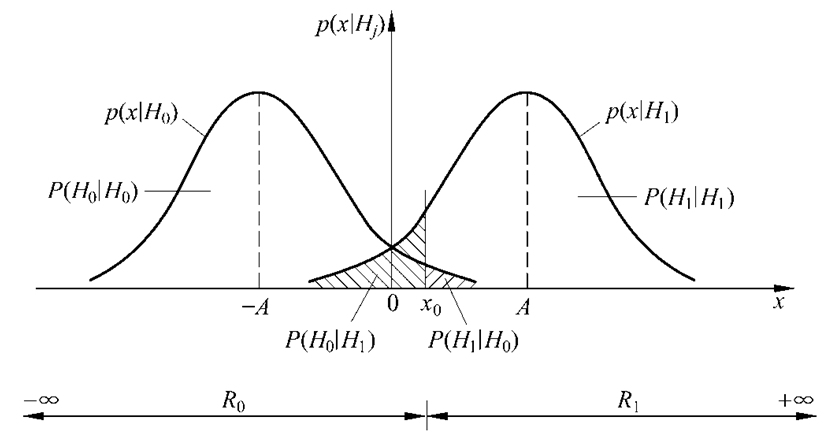
\includegraphics[scale=0.35]{detectionA}
\end{columns}
\begin{align*}
&P({H_1})(c_{01}-c_{11})p(x|H_1)< P(H_0)(c_{10}-c_{00})p(x|H_0)&\textbf{判决$H_0$假设成立}\\
&P({H_1})(c_{01}-c_{11})p(x|H_1)\ge P(H_0)(c_{10}-c_{00})p(x|H_0)&\textbf{判决$H_1$假设成立}
\end{align*}
\end{frame}

\begin{frame}{解决方案}
\begin{enumerate}
	\item 代价因子如何定义? \\
	$c_{ij}$表示假设$H_j$为真时, 判决假设$H_i$成立所付出的代价。\\
	$c_{00}, c_{10}, c_{11}, c_{01}$
	\item 平均代价如何计算?
	\begin{align*}
	C=&P(H_0)C(H_0)+P(H_1)C(H_1)\\
	&c_{10}P(H_0)+c_{11}P(H_1)+\\
	&\left(\int_{R_0}\left[P({H_1})(c_{01}-c_{11})p(x|H_1)-P(H_0)(c_{10}-c_{00})p(x|H_0)\right]dx \right)
	\end{align*}
	\item 如何获得最小的平均代价?
	\begin{align*}
	&P({H_1})(c_{01}-c_{11})p(x|H_1)< P(H_0)(c_{10}-c_{00})p(x|H_0)&\textbf{判决$H_0$假设成立}\\
	&P({H_1})(c_{01}-c_{11})p(x|H_1)\ge P(H_0)(c_{10}-c_{00})p(x|H_0)&\textbf{判决$H_1$假设成立}
	\end{align*}
\end{enumerate}
\end{frame}

\begin{frame}[shrink]{贝叶斯判决准则}
\begin{columns}%[t]
	\column{0.25\textwidth}
	\textbf{二元信号检测模型:}
	\column{0.2\textwidth}
	\begin{align*}
	H_0: &x=-A+n\\
	H_1: &x=A+n
	\end{align*}
	\column{0.35\textwidth}
	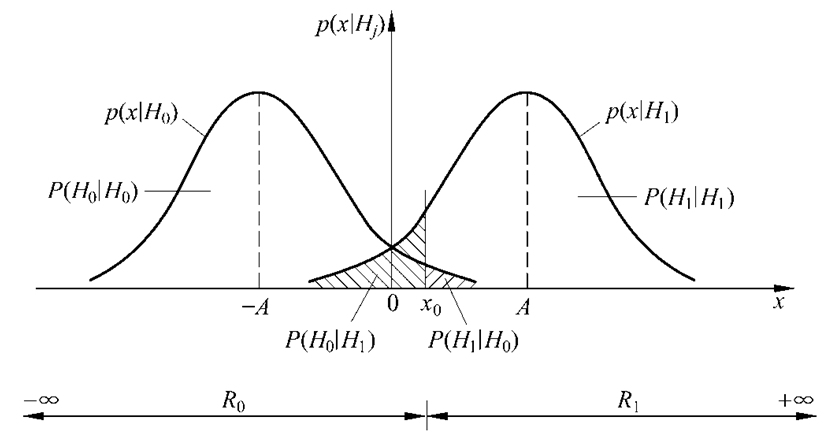
\includegraphics[scale=0.3]{detectionA}
\end{columns}
\begin{align*}
&P({H_1})(c_{01}-c_{11})p(x|H_1)< P(H_0)(c_{10}-c_{00})p(x|H_0)&\textbf{判决$H_0$假设成立}\\
&P({H_1})(c_{01}-c_{11})p(x|H_1)\ge P(H_0)(c_{10}-c_{00})p(x|H_0)&\textbf{判决$H_1$假设成立}
\end{align*}
\begin{block}{贝叶斯判决准则}
	\begin{align*}
	\frac{p(x|H_1)}{p(x|H_0)}&<\frac{P(H_0)(c_{10}-c_{00})}{P(H_1)(c_{01}-c_{11})}&\textbf{判决$H_0$假设成立}\\
	\frac{p(x|H_1)}{p(x|H_0)}&\ge\frac{P(H_0)(c_{10}-c_{00})}{P(H_1)(c_{01}-c_{11})}&\textbf{判决$H_1$假设成立}
	\end{align*}
\end{block}
\end{frame}

\section{贝叶斯准则判决思路}

\begin{frame}{贝叶斯准则判决思路}
\centering
\textcolor{blue}{\textbf{根据给定的代价计算平均代价}}\\
$\Downarrow$\\
\textcolor{blue}{\textbf{按照平均代价最小划分观测空间, 得到判决准则}}\\
$\Downarrow$\\
\textcolor{blue}{\textbf{对判决表达式进行化简}}
\end{frame}

\begin{frame}{贝叶斯判决准则}
\begin{block}{贝叶斯判决准则}
	\begin{align*}
	\frac{p(x|H_1)}{p(x|H_0)}&<\frac{P(H_0)(c_{10}-c_{00})}{P(H_1)(c_{01}-c_{11})}&\textbf{判决$H_0$假设成立}\\
	\frac{p(x|H_1)}{p(x|H_0)}&\ge\frac{P(H_0)(c_{10}-c_{00})}{P(H_1)(c_{01}-c_{11})}&\textbf{判决$H_1$假设成立}
	\end{align*}
	$\implies$
	\[ \frac{p(x|H_1)}{p(x|H_0)}\mathop{\gtrless}_{H_0}^{H_1}\frac{P(H_0)(c_{10}-c_{00})}{P(H_1)(c_{01}-c_{11})} \]
	$\implies$
	\[\lambda(x)\mathop{\gtrless}_{H_0}^{H_1}\eta \]
\end{block}
\end{frame}

\begin{frame}{贝叶斯判决准则}
\begin{block}{贝叶斯判决准则}
	\[ \frac{p(x|H_1)}{p(x|H_0)}\mathop{\gtrless}_{H_0}^{H_1}\frac{P(H_0)(c_{10}-c_{00})}{P(H_1)(c_{01}-c_{11})} \implies \lambda(x)\mathop{\gtrless}_{H_0}^{H_1}\eta \]
	\begin{align*}
	&\lambda(x)\mathop{=}\limits^{def}\frac{p(x|H_1)}{p(x|H_0)} &&\textbf{定义为}\textcolor{blue}{\textbf{似然比函数}}\\
	&\eta\mathop{=}\limits^{def}\frac{P(H_0)(c_{10}-c_{00})}{P(H_1)(c_{01}-c_{11})} &&\textbf{定义为}\textcolor{blue}{定义为\textbf{判决门限}}
	\end{align*}
\end{block}
\textbf{$\lambda(x)$是一维随机变量, 称为\textcolor{blue}{检验统计量}}\\
\textbf{$\lambda(x)$不依赖于假设的先验概率$[P(H_0), P(H_1)]$, 也与代价因子无关。\textcolor{blue}{适用于不同先验概率和不同代价因子的最佳信号检测。}}
\end{frame}

\begin{frame}{贝叶斯准则检测步骤}
\begin{block}{贝叶斯判决准则}
	\[ \frac{p(x|H_1)}{p(x|H_0)}\mathop{\gtrless}_{H_0}^{H_1}\frac{P(H_0)(c_{10}-c_{00})}{P(H_1)(c_{01}-c_{11})} \implies \lambda(x)\mathop{\gtrless}_{H_0}^{H_1}\eta \]
\end{block}
利用贝叶斯判决准则进行检测的基本步骤:
\begin{enumerate}
	\item 计算两个似然函数, 构建似然比$\lambda(x)\mathop{=}\limits^{def}\frac{p(x|H_1)}{p(x|H_0)}$
	\item 根据两个假设的先验概率和代价因子, 计算判决门限$\eta\mathop{=}\limits^{def}\frac{P(H_0)(c_{10}-c_{00})}{P(H_1)(c_{01}-c_{11})}$
	\item 利用上式, 形成贝叶斯检测基本表达式$\lambda(x)\mathop{\gtrless}\limits_{H_0}^{H_1}\eta$
	\item 化简, 如对数似然比检验$\ln\lambda(x)\mathop{\gtrless}\limits_{H_0}^{H_1}\ln\eta\implies l(x)\mathop{\gtrless}\limits_{H_0}^{H_1}\gamma$
\end{enumerate}
\end{frame}

\begin{frame}{二元信号检测系统: $\lambda(x)\mathop{\gtrless}\limits_{H_0}^{H_1}\eta$}
\centering
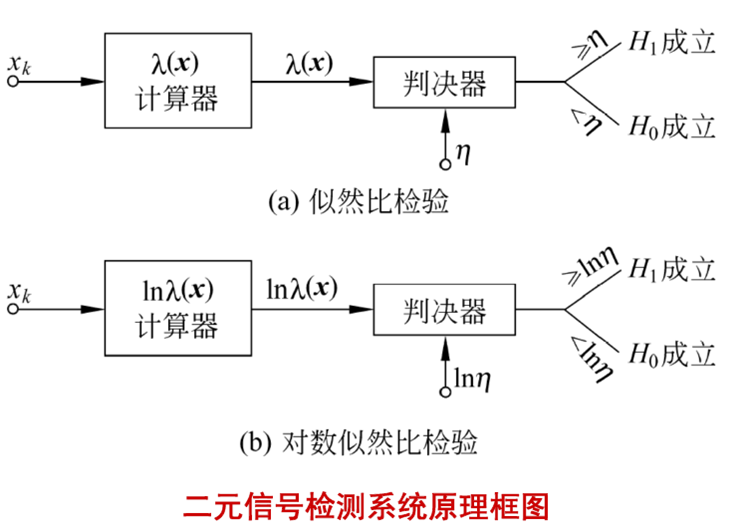
\includegraphics[scale=0.5]{2D}
\end{frame}

\begin{frame}{二元信号检测系统: $\ln\lambda(x)\mathop{\gtrless}\limits_{H_0}^{H_1}\ln\eta\implies l(x)\mathop{\gtrless}\limits_{H_0}^{H_1}\gamma$}
\centering
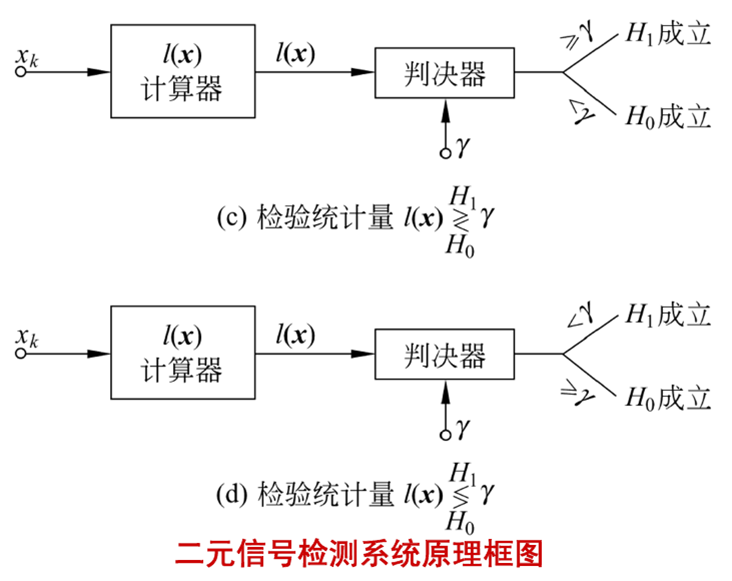
\includegraphics[scale=0.5]{2D2}
\end{frame}

\section{贝叶斯准则小结}

\begin{frame}{贝叶斯准则小结(1)}
\textbf{\textcolor{red}{贝叶斯检测---}\textcolor{blue}{给定各种判决代价因子, 且已知各假设的先验概率条件下, 使\textcolor{red}{平均代价最小}的检测准则。}}\\

\bigskip
\textbf{\textcolor{red}{贝叶斯准则基本思路:}}\\
\centering
\textcolor{blue}{\textbf{根据给定的代价计算平均代价}}\\
$\Downarrow$\\
\textcolor{blue}{\textbf{按照平均代价最小划分观测空间, 得到判决准则}}\\
$\Downarrow$\\
\textcolor{blue}{\textbf{对判决表达式进行化简}}
\end{frame}

\begin{frame}{贝叶斯准则小结(2)}
\textbf{代价因子的定义}
\begin{block}{对于二元信号统计检测, 共有四种事件发生, 即}
	$$
	\begin{array}{cccc}
	(H_0|H_0) & (H_1|H_0) & (H_1|H_1) & (H_0|H_1)\\
	\Downarrow & \Downarrow & \Downarrow & \Downarrow\\
	c_{00} & c_{10} & c_{11} & c_{01}
	\end{array}
	$$
	$c_{ij}$表示假设$H_j$为真时, 判决假设$H_i$成立所付出的代价
\end{block}
\begin{block}{Notes}
	一般地, $c_{10}>c_{00}, c_{01}>c_{11}$
\end{block}
\end{frame}

\begin{frame}[shrink]{贝叶斯准则小结(3)}
\textbf{平均代价取最小的条件}
\begin{align*}
C=&c_{10}P(H_0)+c_{11}P(H_1)+\\
&\left(\int_{R_0}\left[P({H_1})(c_{01}-c_{11})p(x|H_1)-P(H_0)(c_{10}-c_{00})p(x|H_0)\right]dx \right)
\end{align*}
\begin{columns}
	\column{0.46\textwidth}
	\textbf{把被积函数取负值的观测值$x$划分给$R_0$区域, 而把其余的观测值$x$划分给$R_1$, 即可保证平均代价最小。}
	\column{0.35\textwidth}
	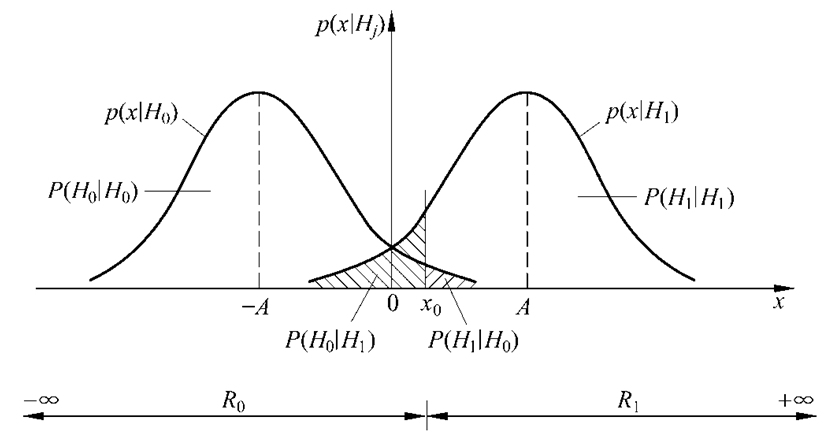
\includegraphics[scale=0.35]{detectionA}
\end{columns}
\begin{align*}
&P({H_1})(c_{01}-c_{11})p(x|H_1)< P(H_0)(c_{10}-c_{00})p(x|H_0)&\textbf{判决$H_0$假设成立}\\
&P({H_1})(c_{01}-c_{11})p(x|H_1)\ge P(H_0)(c_{10}-c_{00})p(x|H_0)&\textbf{判决$H_1$假设成立}
\end{align*}
\end{frame}

\begin{frame}{贝叶斯准则小结(4)}
\begin{block}{贝叶斯判决准则}
	\[ \frac{p(x|H_1)}{p(x|H_0)}\mathop{\gtrless}_{H_0}^{H_1}\frac{P(H_0)(c_{10}-c_{00})}{P(H_1)(c_{01}-c_{11})} \implies \lambda(x)\mathop{\gtrless}_{H_0}^{H_1}\eta \]
	\begin{align*}
	&\lambda(x)\mathop{=}\limits^{def}\frac{p(x|H_1)}{p(x|H_0)} &&\textbf{定义为}\textcolor{blue}{\textbf{似然比函数}}\\
	&\eta\mathop{=}\limits^{def}\frac{P(H_0)(c_{10}-c_{00})}{P(H_1)(c_{01}-c_{11})} &&\textbf{定义为}\textcolor{blue}{定义为\textbf{判决门限}}
	\end{align*}
\end{block}
\textbf{$\lambda(x)$是一维随机变量, 称为\textcolor{blue}{检验统计量}}\\
\textbf{$\lambda(x)$不依赖于假设的先验概率$[P(H_0), P(H_1)]$, 也与代价因子无关。\textcolor{blue}{适用于不同先验概率和不同代价因子的最佳信号检测。}}
\end{frame}

\begin{frame}{贝叶斯准则小结(5)}
\begin{block}{贝叶斯判决准则}
\[ \frac{p(x|H_1)}{p(x|H_0)}\mathop{\gtrless}_{H_0}^{H_1}\frac{P(H_0)(c_{10}-c_{00})}{P(H_1)(c_{01}-c_{11})} \implies \lambda(x)\mathop{\gtrless}_{H_0}^{H_1}\eta \]
\end{block}
利用贝叶斯判决准则进行检测的基本步骤:
\begin{enumerate}
\item 计算两个似然函数, 构建似然比$\lambda(x)\mathop{=}\limits^{def}\frac{p(x|H_1)}{p(x|H_0)}$
\item 根据两个假设的先验概率和代价因子, 计算判决门限$\eta\mathop{=}\limits^{def}\frac{P(H_0)(c_{10}-c_{00})}{P(H_1)(c_{01}-c_{11})}$
\item 利用上式, 形成贝叶斯检测基本表达式$\lambda(x)\mathop{\gtrless}\limits_{H_0}^{H_1}\eta$
\item 化简, 如对数似然比检验$\ln\lambda(x)\mathop{\gtrless}\limits_{H_0}^{H_1}\ln\eta\implies l(x)\mathop{\gtrless}\limits_{H_0}^{H_1}\gamma$
\end{enumerate}
\end{frame}

\section{贝叶斯准则例题}

\begin{frame}{贝叶斯准则例题1}
在二元数字通信系统中,假设为$H_1$时,信源输出为常值正电压$m$, 假设为$H_0$时, 信源输出零电平, 信号在传输过程中迭加了噪声$n(t)$, 每种信号的持续时间为$T$, 请:
\begin{enumerate}
	\item 若接收端对接收信号$x(t)$在$(0,T)$时间内进行1次采样, 给出对应的贝叶斯检测准则。
	\item 若接收端对接收信号$x(t)$在$(0,T)$时间内进行$N$次独立采样, 样本为$x_k(k=1,2,\cdots,N)$。给出对应的贝叶斯检测准则。
\end{enumerate}
上述两种情况下,噪声采样值$n_k$是均值为零,方差为$\sigma_n^2$的高斯噪声。
\end{frame}

\begin{frame}[shrink]{贝叶斯准则例题1: 解}
解: 一次采样时:
\begin{align*}
H_0: x&=n\\
H_1: x&=m+n
\end{align*}
步骤1: 计算两个似然函数, 构建似然比\\
由于$n$是高斯分布随机变量, 因此在$H_0$假设下, 观测信号$x$也服从高斯分布,且均值为0, 方差为$\sigma_n^2$; 在$H_1$假设下, 观测信号$x$服从均值为$m$, 方差为$\sigma_n^2$的高斯分布。
\begin{align*}
p(x|H_0)&=\left(\frac{1}{2\pi\sigma_n^2}\right)^{1/2}\exp\left(-\frac{x^2}{2\sigma_n^2}\right)\\
p(x|H_1)&=\left(\frac{1}{2\pi\sigma_n^2}\right)^{1/2}\exp\left(-\frac{(x-m)^2}{2\sigma_n^2}\right)\\
\lambda(x)&=\frac{p(x|H_1)}{p(x|H_0)}=\exp\left(\frac{x^2-(x-m)^2}{2\sigma_n^2}\right)=\exp\left(\frac{m}{\sigma_n^2}x-\frac{m^2}{2\sigma_n^2}\right)
\end{align*} 
\end{frame}

\begin{frame}[shrink]{贝叶斯准则例题1: 解续(1)}
步骤2: 根据两个假设的先验概率和代价因子, 计算判决门限
\[\eta\mathop{=}\limits^{def}\frac{P(H_0)(c_{10}-c_{00})}{P(H_1)(c_{01}-c_{11})} \]
步骤3: 形成贝叶斯检测基本表达式
\begin{align*}
\lambda(x)&\mathop{\gtrless}\limits_{H_0}^{H_1}\eta\\
\exp\left(\frac{m}{\sigma_n^2}x-\frac{m^2}{2\sigma_n^2}\right)&\mathop{\gtrless}\limits_{H_0}^{H_1}\eta
\end{align*} 
步骤4: 化简
\begin{align*}
%\exp\left(\frac{m}{\sigma_n^2}x-\frac{m^2}{2\sigma_n^2}\right)&\mathop{\gtrless}\limits_{H_0}^{H_1}\eta\\
\left(\frac{m}{\sigma_n^2}x-\frac{m^2}{2\sigma_n^2}\right)&\mathop{\gtrless}\limits_{H_0}^{H_1}\ln\eta\\
l(x)\mathop{=}^{def}x&\mathop{\gtrless}\limits_{H_0}^{H_1}\frac{\sigma_n^2}{m}\ln\eta+\frac{m}{2}\mathop{=}^{def}\gamma\\
\end{align*} 
\end{frame}

\begin{frame}[shrink]{贝叶斯准则例题1: 解续(2)}
\begin{columns}
	\column{0.5\textwidth}
	\begin{align*}
	&&n\sim\mathcal{N}(0,\sigma_n^2)\\ 
	H_0 &:x=n   &x\sim\mathcal{N}(0,\sigma_n^2)\\
	H_1 &:x=m+n &x\sim\mathcal{N}(m,\sigma_n^2)\\
	\end{align*}
	\[\text{判决表达式:  } l(x)\mathop{=}^{def}x\mathop{\gtrless}_{H_0}^{H_1}\frac{\sigma_n^2}{m}\ln\eta+\frac{m}{2}\mathop{=}^{def}\gamma \]
	\column{0.4\textwidth}
	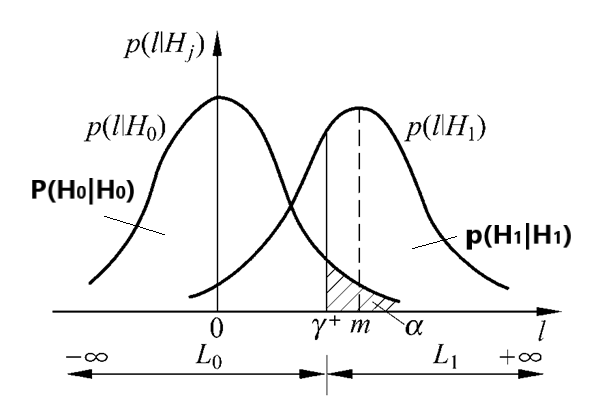
\includegraphics[scale=0.3]{mgt0}\\
	\scriptsize
	\textcolor{blue}{$p(l|H_j)(j=0,1)$: 假设$H_j$下观测信号的概率密度函数; $r^+=\frac{\sigma_n^2}{m}\ln\eta+\frac{m}{2}; \alpha=P(H_1|H_0)$}
\end{columns}
\begin{block}{思考}
	\begin{enumerate}
		\item $\frac{m}{2}$是两个假设的中间值, $\frac{\sigma^2}{m}\ln\eta$为中间值的修正量, 其含义如何?
		\item 考虑$m>0,m<0,m=0$时,如何构造判决表达式?
	\end{enumerate} 
\end{block}
\end{frame}

\begin{frame}[shrink]{贝叶斯准则例题1: 解续(3)}
\begin{enumerate}
	\item $m=0$时: $H_0,H_1$成为一样的噪声信号$n(t)$。
	\item $m\uparrow\implies$ 中间值修正量$(\frac{\sigma^2}{m}\ln\eta)\downarrow$, $\gamma$越接近于中间值$\frac{m}{2}$。
	\item $m$值越大, 更易区分两种假设,检测性能越好。
	\item $m>0$和$m<0$下的判决表达式如下图。
\end{enumerate}	
\begin{columns}
	\column{0.4\textwidth}
	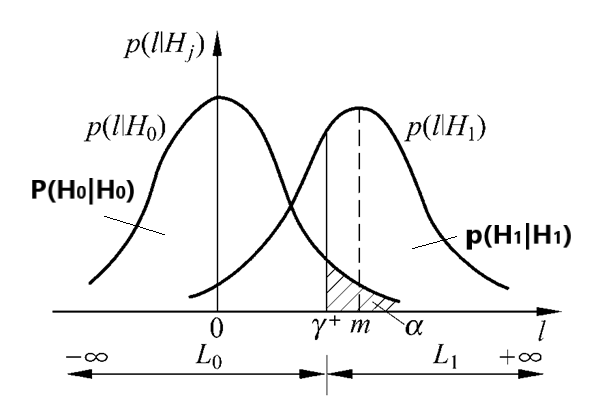
\includegraphics[scale=0.3]{mgt0}
	$m>0;\qquad x\mathop{\gtrless}\limits_{H_0}^{H_1}\frac{\sigma^2}{m}\ln\eta+\frac{m}{2}$
	\column{0.4\textwidth}
	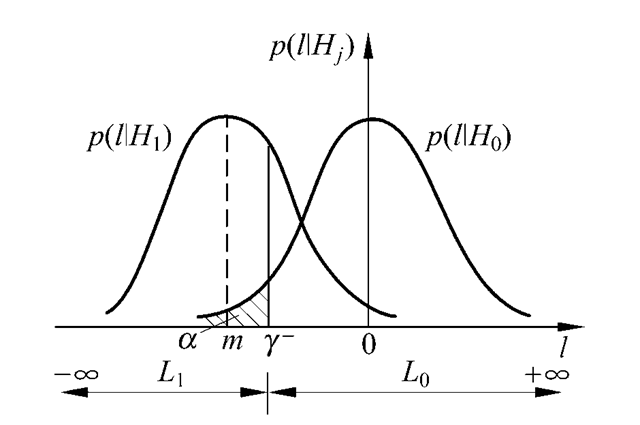
\includegraphics[scale=0.45]{mle0}
	$m<0;\qquad x\mathop{\lessgtr}\limits_{H_0}^{H_1}-\frac{\sigma^2}{|m|}\ln\eta-\frac{|m|}{2}$
\end{columns}
\end{frame}

\begin{frame}[shrink]{贝叶斯准则例题1: 解续(4)}
解: $N$次独立采样, 样本为$x_k(k=1,2,\cdots,N)$:
\begin{align*}
H_0: x_k&=n_k && x_k(k=1,2,\cdots,N)\\
H_1: x_k&=m+n_k && x_k(k=1,2,\cdots,N)
\end{align*}
步骤1: 计算两个似然函数, 构建似然比\\
由于$n$是高斯分布随机变量, 因此在$H_0$假设下, 第$k$次采样值$x_k$服从高斯分布,且均值为0, 方差为$\sigma_n^2$; 在$H_1$假设下, 第$k$次采样值$x_k$服从均值为$m$, 方差为$\sigma_n^2$的高斯分布。
\begin{align*}
p(x_k|H_0)&=\left(\frac{1}{2\pi\sigma_n^2}\right)^{1/2}\exp\left(-\frac{x_k^2}{2\sigma_n^2}\right)\implies p(\bm{x}|H_0)=\prod_{k=1}^{N}\left(\frac{1}{2\pi\sigma_n^2}\right)^{1/2}\exp\left(-\frac{x_k^2}{2\sigma_n^2}\right)\\
p(x_k|H_1)&=\left(\frac{1}{2\pi\sigma_n^2}\right)^{1/2}\exp\left(-\frac{(x-m)^2}{2\sigma_n^2}\right)\implies p(\bm{x}|H_1)=\prod_{k=1}^{N}\left(\frac{1}{2\pi\sigma_n^2}\right)^{1/2}\exp\left(-\frac{(x_k-m)^2}{2\sigma_n^2}\right)\\
\lambda(\bm{x})&=\frac{p(\bm{x}|H_1)}{p(\bm{x}|H_0)}=\exp\left(\frac{\sum\limits_{k=1}^{N}(x_k^2-(x_k-m)^2)}{2\sigma_n^2}\right)
\end{align*} 
\end{frame}

\begin{frame}[shrink]{贝叶斯准则例题1: 解续(5)}
步骤2: 根据两个假设的先验概率和代价因子, 计算判决门限
\[\eta\mathop{=}\limits^{def}\frac{P(H_0)(c_{10}-c_{00})}{P(H_1)(c_{01}-c_{11})} \]
步骤3: 形成贝叶斯检测基本表达式
\begin{align*}
\lambda(x)&\mathop{\gtrless}\limits_{H_0}^{H_1}\eta\\
\exp\left(\frac{\sum\limits_{k=1}^{N}(x_k^2-(x_k-m)^2)}{2\sigma_n^2}\right)&\mathop{\gtrless}\limits_{H_0}^{H_1}\eta
\end{align*} 
步骤4: 化简
\begin{align*}
-Nm^2+\sum\limits_{k=1}^{N}2mx_k&\mathop{\gtrless}\limits_{H_0}^{H_1}2\sigma_n^2\ln\eta\implies \sum\limits_{k=1}^{N}x_k\mathop{\gtrless}\limits_{H_0}^{H_1}\frac{\sigma_n^2}{m}\ln\eta+\frac{Nm}{2}\\
l(\bm{x})\mathop{=}^{def}\frac{1}{N}\sum\limits_{k=1}^{N}x_k&\mathop{\gtrless}\limits_{H_0}^{H_1}\frac{\sigma_n^2}{Nm}\ln\eta+\frac{m}{2}\mathop{=}^{def}\gamma\\
\end{align*} 
\end{frame}

\begin{frame}[shrink]{贝叶斯准则例题1: 解续(6)}
经过上述化简, 信号检测的判决式由似然比检验的形式, 简化为检验统计量$l(x)$与检测门限$\gamma$相比较的形式, 形成贝叶斯检测判决表达式:
\[
l(\bm{x})\mathop{=}^{def}\frac{1}{N}\sum\limits_{k=1}^{N}x_k\mathop{\gtrless}\limits_{H_0}^{H_1}\frac{\sigma_n^2}{Nm}\ln\eta+\frac{m}{2}\mathop{=}^{def}\gamma
\]
检验统计量$l(x)\mathop{=}\limits^{def}\frac{1}{N}\sum\limits_{k=1}^Nx_k$是观测信号$x_k(k=1,2,\dots,N)$的求和取平均值的结果, 即它是$x_k(k=1,2,\dots,N)$的函数,是一个随机变量。\\
因为高斯随机变量的线性组合还是高斯随机变量,  所以两种假设下的观测量$(l|H_0),(l|H_1)$也是服从高斯分布的随机变量。
\end{frame}

\begin{frame}[shrink]{贝叶斯准则例题1: 解续(7)}
$N$次独立采样, 样本为$x_k(k=1,2,\dots,N)$
\begin{align*}
	&&n_k\sim\mathcal{N}(0,\sigma_n^2)\\ 
	H_0 &:x_k=n_k   &(l|H_0)\sim\mathcal{N}(0,\frac{\sigma_n^2}{N})\\
	H_1 &:x_k=m+n_k &(l|H_1)\sim\mathcal{N}(m,\frac{\sigma_n^2}{N})
\end{align*}
\begin{columns}
\column{0.4\textwidth}	
\textbf{贝叶斯检测判决表达式:}\\
\[
l(\bm{x})\mathop{=}^{def}\frac{1}{N}\sum\limits_{k=1}^{N}x_k\mathop{\gtrless}\limits_{H_0}^{H_1}\frac{\sigma_n^2}{Nm}\ln\eta+\frac{m}{2}\mathop{=}^{def}\gamma
\]
\column{0.4\textwidth}
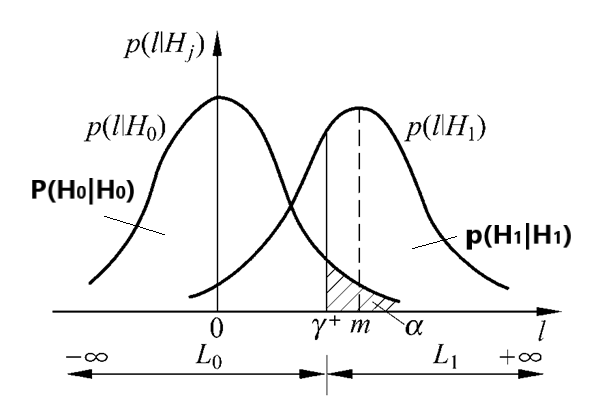
\includegraphics[scale=0.25]{mgt0}\\
\scriptsize
\textcolor{blue}{$p(l|H_j)(j=0,1)$: 假设$H_j$下观测信号的概率密度函数; $r^+=\frac{\sigma^2\ln\eta}{Nm}+\frac{m}{2}; \alpha=P(H_1|H_0)$}
\end{columns}
\end{frame}



